\begin{figure}[!ht]
	\centering
	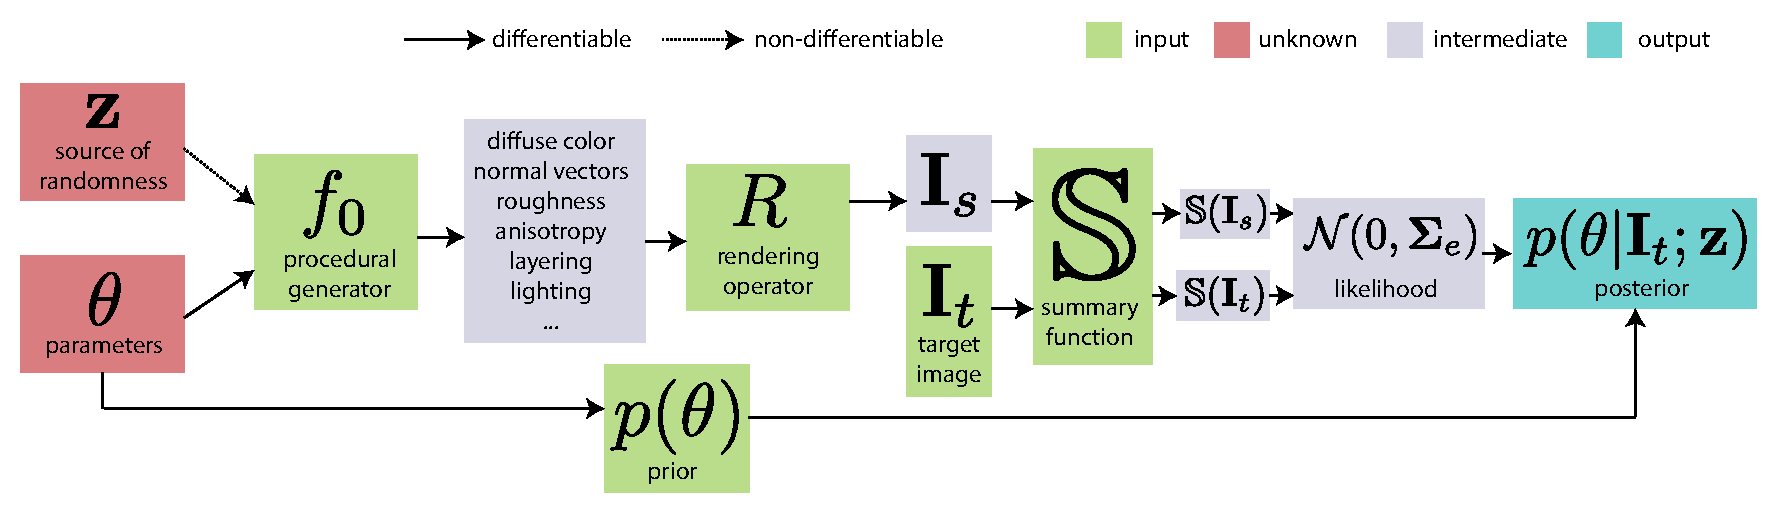
\includegraphics[width=\textwidth]{bayesian/fig1-2/posterior.pdf}
	\caption[Pipeline]{\label{fig:bayesian:pipeline}
		Our posterior computation combines priors, a procedural material model, a rendering operator, a summary function, and a target image. This posterior distribution can then be sampled to provide plausible values of the parameter vector. The value of the posterior is computed up to a normalization term, which does not effect MCMC sampling. The entire posterior definition is differentiable in the material parameters (excluding optional discrete model parameters).}
\end{figure}